
\subsection{Non-linear separability}

\begin{frame}

\question{What about non-linearly separable classes?}

\only<1>{

	\begin{figure}[h]
		\centering
		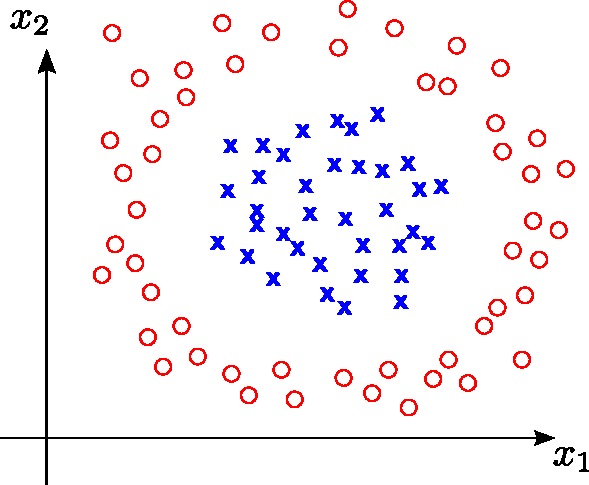
\includegraphics[height=4.5cm]{img/circular} 
		\mode<article>{
		\caption{
		A non-linearly separable case.
		}
		\label{fig:conditionsv}
		} 
	\end{figure}
}

\pause

- Feature transformation.
\notesonly{
The feature space is transformed into a new space in which the classes can become linearly separable:
}
			\begin{equation}
				\underbrace{ \vec{x} }_{\substack{\text{elementary} \\
								\text{features}}}
				\longrightarrow \underbrace{ \vec{\phi}_{(\vec{x})} }_{
						\substack{ \text{monomials of}\\ \text{degree $n$}}}
			\end{equation}
\notesonly{
However, instead of computing the transformation $\vec \phi$ explicitly (possibly very costly in terms of memory footprint if the space of $\vec \phi$ has a very high dimensionality), we exploit the fact that }SVMs only ever operate with the scalar product. This is evident from the Lagrangian of the dual problem we use to construct the SVM:

\begin{equation} 
    L(\{\lambda_\alpha\})
        \;\;=\;\;  -\frac{1}{2} \sum\limits_{\alpha, \beta = 1}^p 
        \lambda_\alpha \lambda_\beta y_T^{(\alpha)}
        y_T^{(\beta)} 
        \underbrace{\big( \vec{x}^{(\alpha)} \big)^\top 
            \vec{x}^{(\beta)}}_{ \circledast }
        + \sum\limits_{\alpha = 1}^p \lambda_\alpha{}
        \eqexcl \max_{\{\lambda_\alpha\}}
\end{equation}	

A transformation of the features would result in:

\slidesonly{\vspace{-3mm}}
\begin{equation} 
    L(\{\lambda_\alpha\})
        \;\;=\;\;  -\frac{1}{2} \sum\limits_{\alpha, \beta = 1}^p 
        \lambda_\alpha \lambda_\beta y_T^{(\alpha)}
        y_T^{(\beta)} 
        \underbrace{\big( \vec \phi_{\vec{x}^{(\alpha)}} \big)^\top 
            \vec \phi_{\vec{x}^{(\beta)}}}_{ \circledast }
        + \sum\limits_{\alpha = 1}^p \lambda_\alpha{}
        \eqexcl \max_{\{\lambda_\alpha\}}
\end{equation}
    
\end{frame}

\subsubsection{Typical kernel functions}

\begin{frame}\frametitle{\subsubsecname}
	\[ \begin{array}{ll}
		K_{(\vec{x}, \vec{x}')} = \big( \vec{x}^\top \vec{x}' + 1 \big)^d
		& \text{polynomial kernel of degree } d\\ 
		& \rightarrow \text{ image processing: pixel correlations} \\[4mm]
		K_{(\vec{x}, \vec{x}')} = \exp \Big\{ -\frac{(\vec{x} - \vec{x}')^2}{
			2 \sigma^2} \Big\}
		& \text{RBF-kernel with range } \sigma \\[-1mm]  
		& \rightarrow \text{ infinite dimensional feature space} \\[4mm]
		K_{(\vec{x}, \vec{x}')} = \tanh \big\{ \kappa \vec{x}^\top \vec{x}' + \theta
			\big\}
		& \text{neural network kernel with parameters } \\ 
		&	\kappa \text{ and } \theta 
			\rightarrow \text{ not positive definite} \\[4mm]
		K_{(\vec{x}, \vec{x}')} = \frac{1}{ (\|\vec{x} - \vec{x}'\|^2 
			+ \epsilon^2 )^{N/2}}
		& \text{Plummer kernel with parameter } \epsilon \\[-1mm]
		& \rightarrow \text{ scale invariant kernel}
	\end{array} \]
\end{frame}

\begin{frame}\frametitle{Induced feature space}
	$$
			K(\vec x, \vec x') 
			%\quad=\quad \sum_{i=0}^{\infty} \,
			%\lambda_i \; \psi_{i(\vec x)} \, \psi_{i(\vec x')} 
			\quad=\quad 
			\sum_{i=1}^{\infty} \,
			\underbrace{\psi_{i(\vec x)} \, \sqrt{\lambda_i}}_{\phi_{i(\vec x)}}
			\underbrace{\sqrt{\lambda_i} \, \psi_{i(\vec x')} }_{\phi_{i(\vec x')}} 
			\quad=\quad \vec \phi_{(\vec x)}^\top \vec \phi_{(\vec x')}
	$$

	\begin{itemize}
		\item every positive semi-definite kernel $K$
			is an \textbf{inner product} in the induced space $\Phi$,
			spanned by the features
			$\phi_{i(\vec x)} = \sqrt{\lambda_i} \, \psi_{i(\vec x)}$
		\vspace{4mm}
		\item $\Phi$ is often high dimensional
		\vspace{4mm}
		\item a linear classifier in $\Phi$ can solve 
			non-linearly separable problems in the original feature space $\Set X$
	\end{itemize}
\end{frame}

\begin{frame}\frametitle{The Gram (``Kernel'') matrix}

The Lagrangian of the dual problem for transformed features involves computing $\big( \vec \phi_{\vec{x}^{(\alpha)}} \big)^\top 
            \vec \phi_{\vec{x}^{(\beta)}}$ for all $\alpha,\beta=1,\ldots,p$, i.e. all pairs of training points:

\begin{equation} 
    L(\{\lambda_\alpha\})
        \;\;=\;\;  -\frac{1}{2} \sum\limits_{\alpha, \beta = 1}^p 
        \lambda_\alpha \lambda_\beta y_T^{(\alpha)}
        y_T^{(\beta)} 
        \underbrace{\big( \vec \phi_{\vec{x}^{(\alpha)}} \big)^\top 
            \vec \phi_{\vec{x}^{(\beta)}}}_{ K(\vec{x}^{(\alpha)}, \vec{x}^{(\beta)})  }
        + \sum\limits_{\alpha = 1}^p \lambda_\alpha{}
        \eqexcl \max_{\{\lambda_\alpha\}}
\end{equation}

\notesonly{This suggests the construction of the Gram matrix $\vec K$:}

\begin{block}{The Gram matrix $\vec K$} 
		$K_{\alpha\beta} = K_{(\vec{x}^{(\alpha)}, \vec{x}^{(\beta)})}$
		\hspace{1cm}
		$\begin{array}{c|ccccc}
		  & 1      & 2      & 3      & \ldots & j      \\
		  \hline
		  1	& K_{11} & K_{12} & \ldots & \ldots & K_{1j} \\
		  2 	& \vdots & \vdots & K_{23} & \ldots & K_{2j} \\
		  \vdots 	& \vdots & \vdots & \vdots & \vdots & \vdots \\
		  i	& K_{i1} & K_{i2} & \ldots & \ldots & K_{ij}
		\end{array}
		$
	\end{block}
	

\question{what are the advantages/disadvantages of constructing the matrix $\vec K$}

\pause

\notesonly{
- Constructing the matrix has the advantage of parallelizing applying the kernel on all the different pairs to speed up computation.
However, it requires the storage of $p \times p$ values, which could be costly if the number of training points $p$ is very large.
}

\end{frame}

\begin{frame}\frametitle{RBF Kernel}

\question{What can we say about entries in $\vec K$ if we select a radial basis function (RBF)/Gaussian kernel?}

\mode<presentation>{

		$$\begin{array}{c|ccccc}
		  & 1      & 2      & 3      & \ldots & j      \\
		  \hline
		  1	& K_{11} & K_{12} & \ldots & \ldots & K_{1j} \\
		  2 	& \vdots & \vdots & K_{23} & \ldots & K_{2j} \\
		  \vdots 	& \vdots & \vdots & \vdots & \vdots & \vdots \\
		  i	& K_{i1} & K_{i2} & \ldots & \ldots & K_{ij}
		\end{array}
		$$
}

\end{frame}

\subsubsection{SVM-RBF vs. RBF networks}

\begin{frame}\frametitle{\subsubsecname}
	
\slidesonly{\vspace{-4mm}}
\begin{figure}[h]
     \centering
     \savebox{\imagebox}{
	 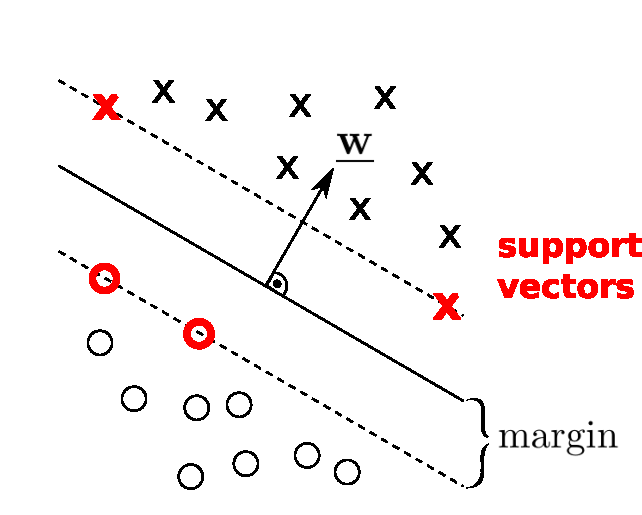
\includegraphics[width=0.35\textwidth]{img/section2_fig18_sv_legend_nolambda}}%
     \begin{subfigure}[t]{0.35\textwidth}
         \centering
         \usebox{\imagebox}% Place largest image
         \mode<article>{
         \caption{
		SVM for classification for classification}
         }
     \end{subfigure}
     \hspace{3mm}
     \begin{subfigure}[t]{0.35\textwidth}
         \centering
         \raisebox{\dimexpr.5\ht\imagebox-.5\height}{% Raise smaller image into place
         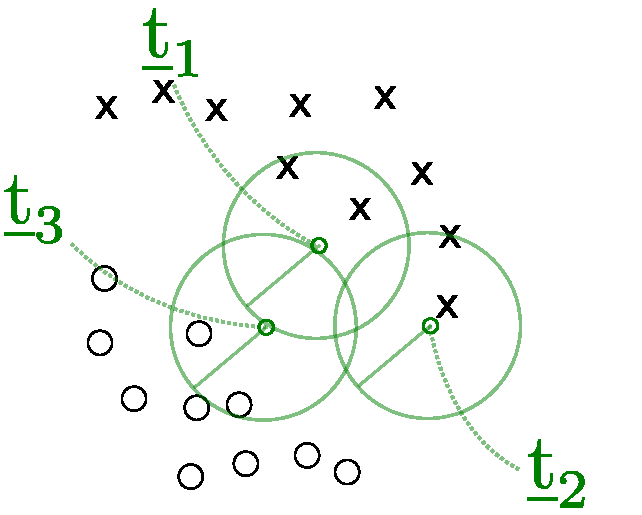
\includegraphics[width=0.99\textwidth]{img/section2_fig18_sv_legend_nolambda_rbf}
         }
         \mode<article>{
         \caption{
		RBF-network for classification}
         }
     \end{subfigure}
	 \label{fig:svmvsrbf}
\end{figure}
	
\slidesonly{\vspace{-2mm}}

\begin{itemize}
			\item \notesonly{Recall how an RBF network can be used for classification:\\}
			
			e.g. \slidesonly{RBF-network with} $3$ centroids \slidesonly{$\vec t_i$}, $i = 1,\ldots,3$
			
			{\footnotesize $$
				y(\vec x) 
				= \sign\Big( \smallsum{i=1}{3} \,
					w_i \exp\kern-.5ex\big(\smallfrac{1}{2\sigma_i^2} 
						\|\vec x - \vec t_i \|^2\big) \Big)
			$$ }
			\notesonly{
			where $\vec t_i$ denotes the coordinates of the $i$-th centroid.
			}
			\item \notesonly{Comparing this to an SVM with a Gaussian kernel, } SVM-RBF:
			
\slidesonly{\vspace{-3mm}}
			{\footnotesize $$
				y(\vec x) 
				= \sign\Big(\smallsum{\alpha \in \mathrm{SV}}{} 
				\lambda_\alpha y_T^{(\alpha)}
					\exp\kern-.5ex\big(\smallfrac{1}{2\sigma^2} 
						\|\vec x - \vec x^{(\alpha)} \|^2\big)
			 	+ b \Big)
			$$ }

\question{How can we conceptually turn an RBF-network into an SVM-RBF}

\notesonly{
- A rough outline of doing so would entail: 
\begin{enumerate}
\item defining as many centroids to match the number of support vectors,
\item placing the centroids on top of the support vectors,
\item find $\vec w$ such that the margin is maximized
\end{enumerate}
}

\end{itemize}

\end{frame}


